\documentclass[final, usenames, dvipsnames]{beamer}
\mode<presentation>{\usetheme{GWU}}
\usepackage{poster_packages}
\usepackage{tikz_packages}
\tdplotsetmaincoords{60}{125} % view angle in spherical coordinates
\input{my_macros}

\DeclareSIUnit\year{yr}

\usepackage[orientation=landscape, width=121.92cm, height=91.44cm,scale=1.24,debug]{beamerposter} 
% \beamertemplategridbackground[1cm] % grid for aligning stuff

%\setlength{\abovecaptionskip}{0.1cm}
%\setlength{\belowcaptionskip}{-0.3cm}

\def\newblock{} % Avoid the "\newblock undefined" error. See http://newsgroups.derkeiler.com/Archive/Comp/comp.text.tex/2008-07/msg00381.html"

%-----------------------------------------------------------
\newlength{\colsep}
\newlength{\onecolwidth}
\newlength{\twocolwidth}

\setlength{\paperwidth}{121.92cm} % 48in
\setlength{\paperheight}{91.44cm} % 36in


%\setlength{\onecolwidth}{0.23\textwidth} % Width of one column
%\setlength{\twocolwidth}{0.49\textwidth} % Width of two columns
\setlength{\onecolwidth}{28cm} % Width of one column
\setlength{\twocolwidth}{56cm} % Width of two columns
\newlength{\columnheight}
\setlength{\columnheight}{76.5cm}

\setbeamersize{text margin left=1.5cm,text margin right=0.5cm}

\listfiles

%-----------------------------
% MACROS
%-----------------------------
\def\Emph{\textcolor{RoyalBlue}}
%%%%%%%%%%%%%%%%%%%%%%%%%%%%%%%%%%%%%%%%%%%%%%%%%%%%%%%%%%%%%%%%%%%%%%%%%%%%%%%%%%%%%%
%	TITLE
%%%%%%%%%%%%%%%%%%%%%%%%%%%%%%%%%%%%%%%%%%%%%%%%%%%%%%%%%%%%%%%%%%%%%%%%%%%%%%%%%%%%%%%
\title{\Large Spacecraft Trajectory Design Near Asteroid 4769 Castalia}
\author{\Large \textcolor{white}{Shankar Kulumani}}
\institute{\large Flight Dynamics and Controls Laboratory (Dr. Taeyoung Lee)\\Department of Mechanical and Aerospace Engineering, School of Engineering and Applied Science}

%----------------------------------------------------------------------------------------

\begin{document}
\begin{frame}[t] % enclose entire poster in a frame
\begin{columns}[T,onlytextwidth] % start of all columns in poster

%-----------------------------------------------------------------------------------------
% FIRST (LEFT) COLUMN
%---------------------------------------------------------------------------------------
\begin{column}{\onecolwidth} % first column start

\begin{block}{Introduction} % Background block
	\begin{itemize}
		\item Asteroids and comets are of significant interest 
		\begin{itemize}
			\item \Emph{Science} - Insight into early solar system formation
			\item \Emph{Mining} - vast quantities of useful materials
			\item \Emph{Impact} - high risk from hazardous Near-Earth asteroids
		\end{itemize}
		\item Near-Earth asteroids (NEAs) are especially interesting 
		\begin{itemize}
			\item Orbit close to the Earth and are easily accessible
			\item Many asteroids hold vast quantities of useful materials
			\item Asteroid mining: Precious metals, propulsion fuels, semiconductors
			\item Commercialization is feasible with huge amounts of possible profit 
		\end{itemize}
		\item High probability of future asteroid impacts
	\end{itemize}
	\vspace{0.2in}
	\begin{figure}
        \begin{subfigure}[b]{0.4\columnwidth}%
	        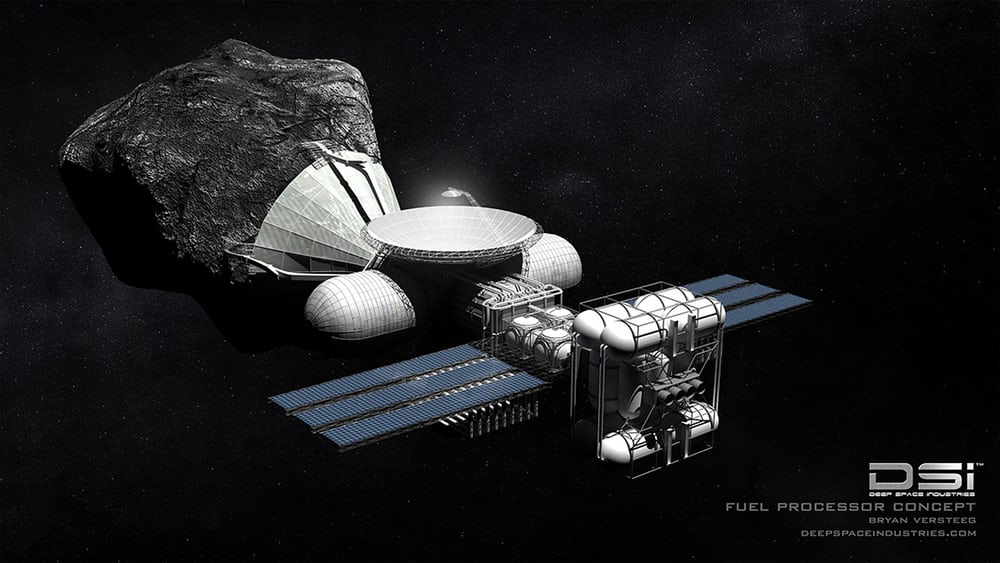
\includegraphics[height=8.5cm]{figures/asteroid-mining-feature-8.jpg}%
	        \caption*{Asteroid Mining}%
        \end{subfigure}~\hfill 
        \begin{subfigure}[b]{0.4\columnwidth}%
            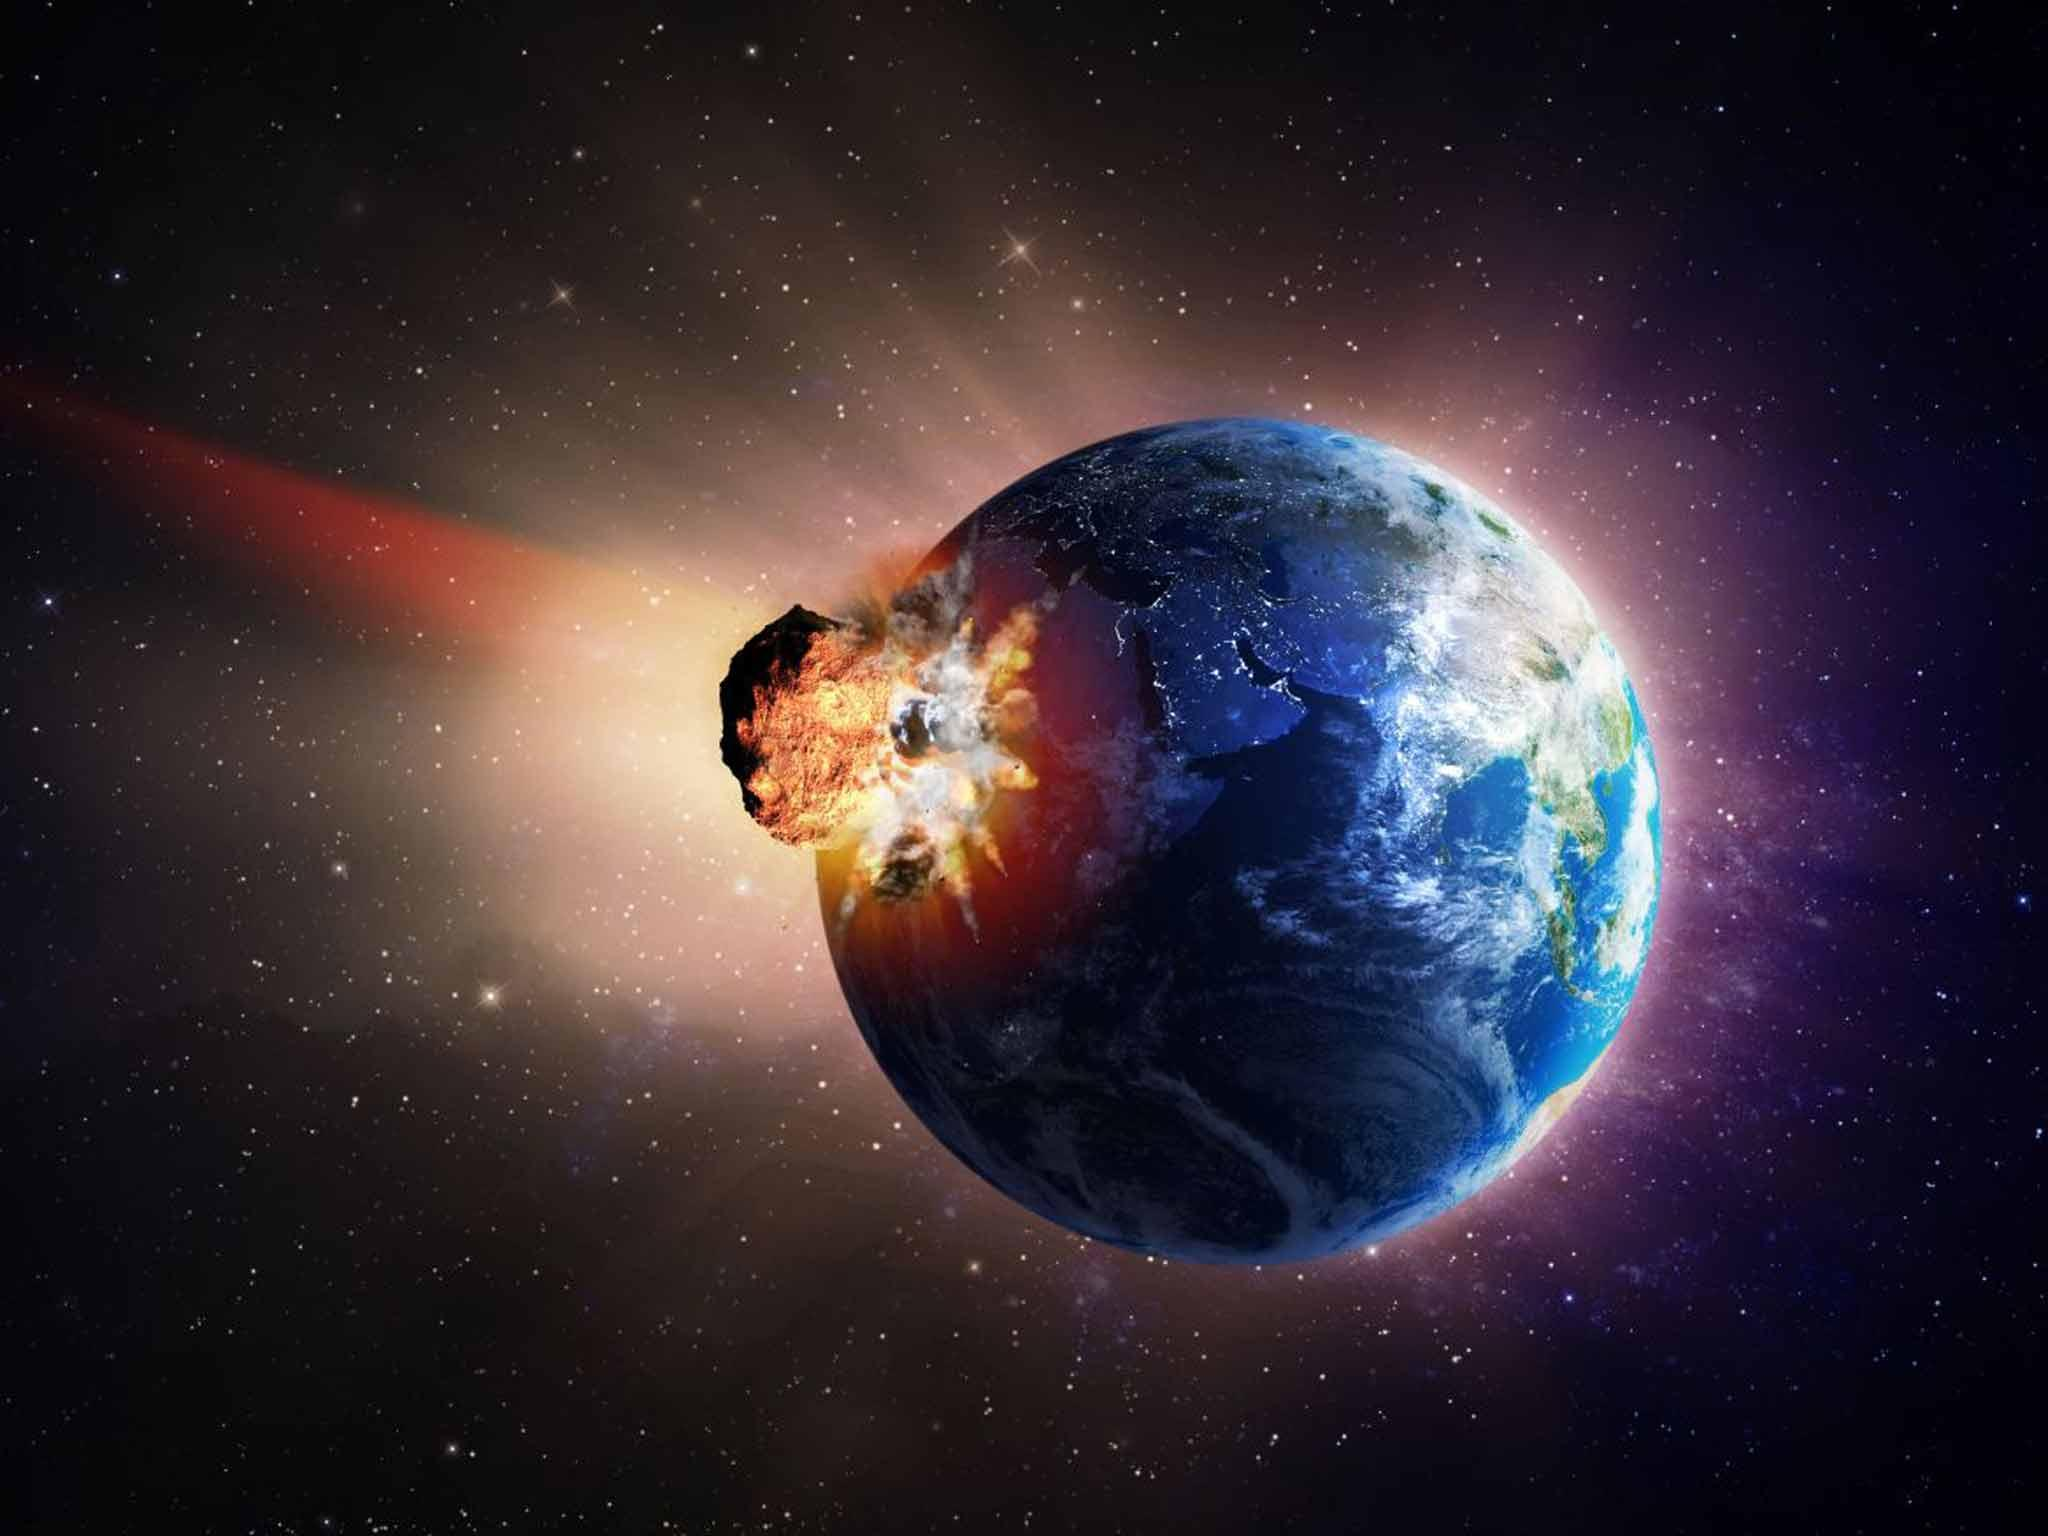
\includegraphics[height=8.5cm]{figures/asteroid-alamy.jpg}%
            \caption*{Asteroid Impact}%
        \end{subfigure}%
        \hfill%
	\end{figure}
\end{block} % end of background block

\begin{block}{Technical Challenges}
	\begin{itemize}
		\item Low-thrust propulsion systems offer innovative options
		\begin{itemize}
			\item Electric propulsion offers much greater efficiency
			\item Allows for greater velocity change with a reduced mass cost
			\item Key component for long duration missions with frequent thrusting
			\item Requires new methods of design
		\end{itemize}
		\item Optimal trajectory design is complicated
		\begin{itemize}
			\item Highly nonlinear and chaotic dynamics requires intuition by designer
			\item Using low-thrust propulsion adds additional difficulties in accurately capturing the small perturbations
		\end{itemize}
		\item Astrodynamic trajectory design typically uses direct optimal control
		\begin{itemize}
			\item Large nonlinear programming problem inherently approximates the true optimal solution
			\item High dimensionality of the solution makes it extremely computationally intensive
		\end{itemize}
	\end{itemize}
\end{block} 

\begin{block}{Gravitational Modeling}
	\begin{itemize}
		\item Asteroids are extended bodies - not point masses
		\begin{itemize}
			\item Gravity is the key force in orbital mechanics
			\item An accurate representation of gravity is critical to accurate and realistic analysis
		\end{itemize}
		\item Spherical Harmonic approach is popular but not ideal
		\begin{itemize}
			\item Model is only valid outside of circumscribing sphere
			\item Composed of an infinite series - always results in an approximation
			\item Model will diverge when close to the surface and is not ideal for landing missions
		\end{itemize}
		\item \Emph{Polyhedron Gravitational model} used to represent the asteroid
		\begin{itemize}
			\item Gravity is a function of the shape model
			\item Globally valid and closed-form analytical solution for gravity
			\item Exact potential assumes a constant density assumption
			\item Accuracy is only dependent on the shape
		\end{itemize}
	\end{itemize}
	\[
	U(\vecbf{r}) &= \frac{1}{2} G \sigma \sum_{e \in \text{edges}} \vecbf{r}_e \cdot \vecbf{E}_e \cdot \vecbf{r}_e \cdot L_e - \frac{1}{2}G \sigma \sum_{f \in \text{faces}} \vecbf{r}_f \cdot \vecbf{F}_f \cdot \vecbf{r}_f \cdot \omega_f 
	\]	
\end{block} 

\end{column}  % first column end

%-----------------------------------------------------------------------------------------
% SECOND (WIDE MIDDLE) COLUMN
%---------------------------------------------------------------------------------------
\begin{column}{\twocolwidth} % second column start

\begin{block}{Dynamics about the asteroid 4769 Castalia} % structure block
	\begin{minipage}{0.5\columnwidth} % left half of this block
	\begin{itemize}
		\item Dynamics are very similar to the famous three-body problem
			\[
			\begin{bmatrix} \dot{\vecbf{r}} \\ \dot{\vecbf{v}} \end{bmatrix} =
			\begin{bmatrix}\vecbf{v} \\ \vecbf{g} \parenth{\vecbf{r}} + \vecbf{h}\parenth{\vecbf{v}} + \vecbf{u} \end{bmatrix} 
			\]
		\item Huge history of analytical tools allow for great insight into the dynamics
		\item Analytical insight is critical to understanding the free motion around an asteroid
		\begin{itemize}
			\item We require an accurate understanding of the motion under the influence of gravity alone
			\item Efficient use of the limited oboard fuel is dependent on exploiting the natural dynamics of the asteroid environment
		\end{itemize}
		\item Jacobi Integral - single constant of motion which bounds the feasible regions in terms of ``energy''
			\[
			J \parenth{\vecbf{r}, \vecbf{v}} = \frac{1}{2} \omega^2 \parenth{x^2 + y^2} + U(\vecbf{r}) - \frac{1}{2} \parenth{\dot{x}^2 + \dot{y}^2 + \dot{z}^2} 
			\]
	\end{itemize}
	\end{minipage}% end of left half of block
	\begin{minipage}{0.5\columnwidth}% right half of block
        \begin{itemize}
            \item Spacecraft is operating around \Emph{4769 Castalia}
            \begin{itemize}
                \item Discovered in 1989, Castalia is a potentially hazardous asteroid and passes close to the Earth
                \item In 1989, Castalia passed close enough to allow for high resolution radar imagery
                \item High resolution shape is used in \Emph{polyhedral gravity model}
            \end{itemize}
        \end{itemize}
		\begin{figure}
			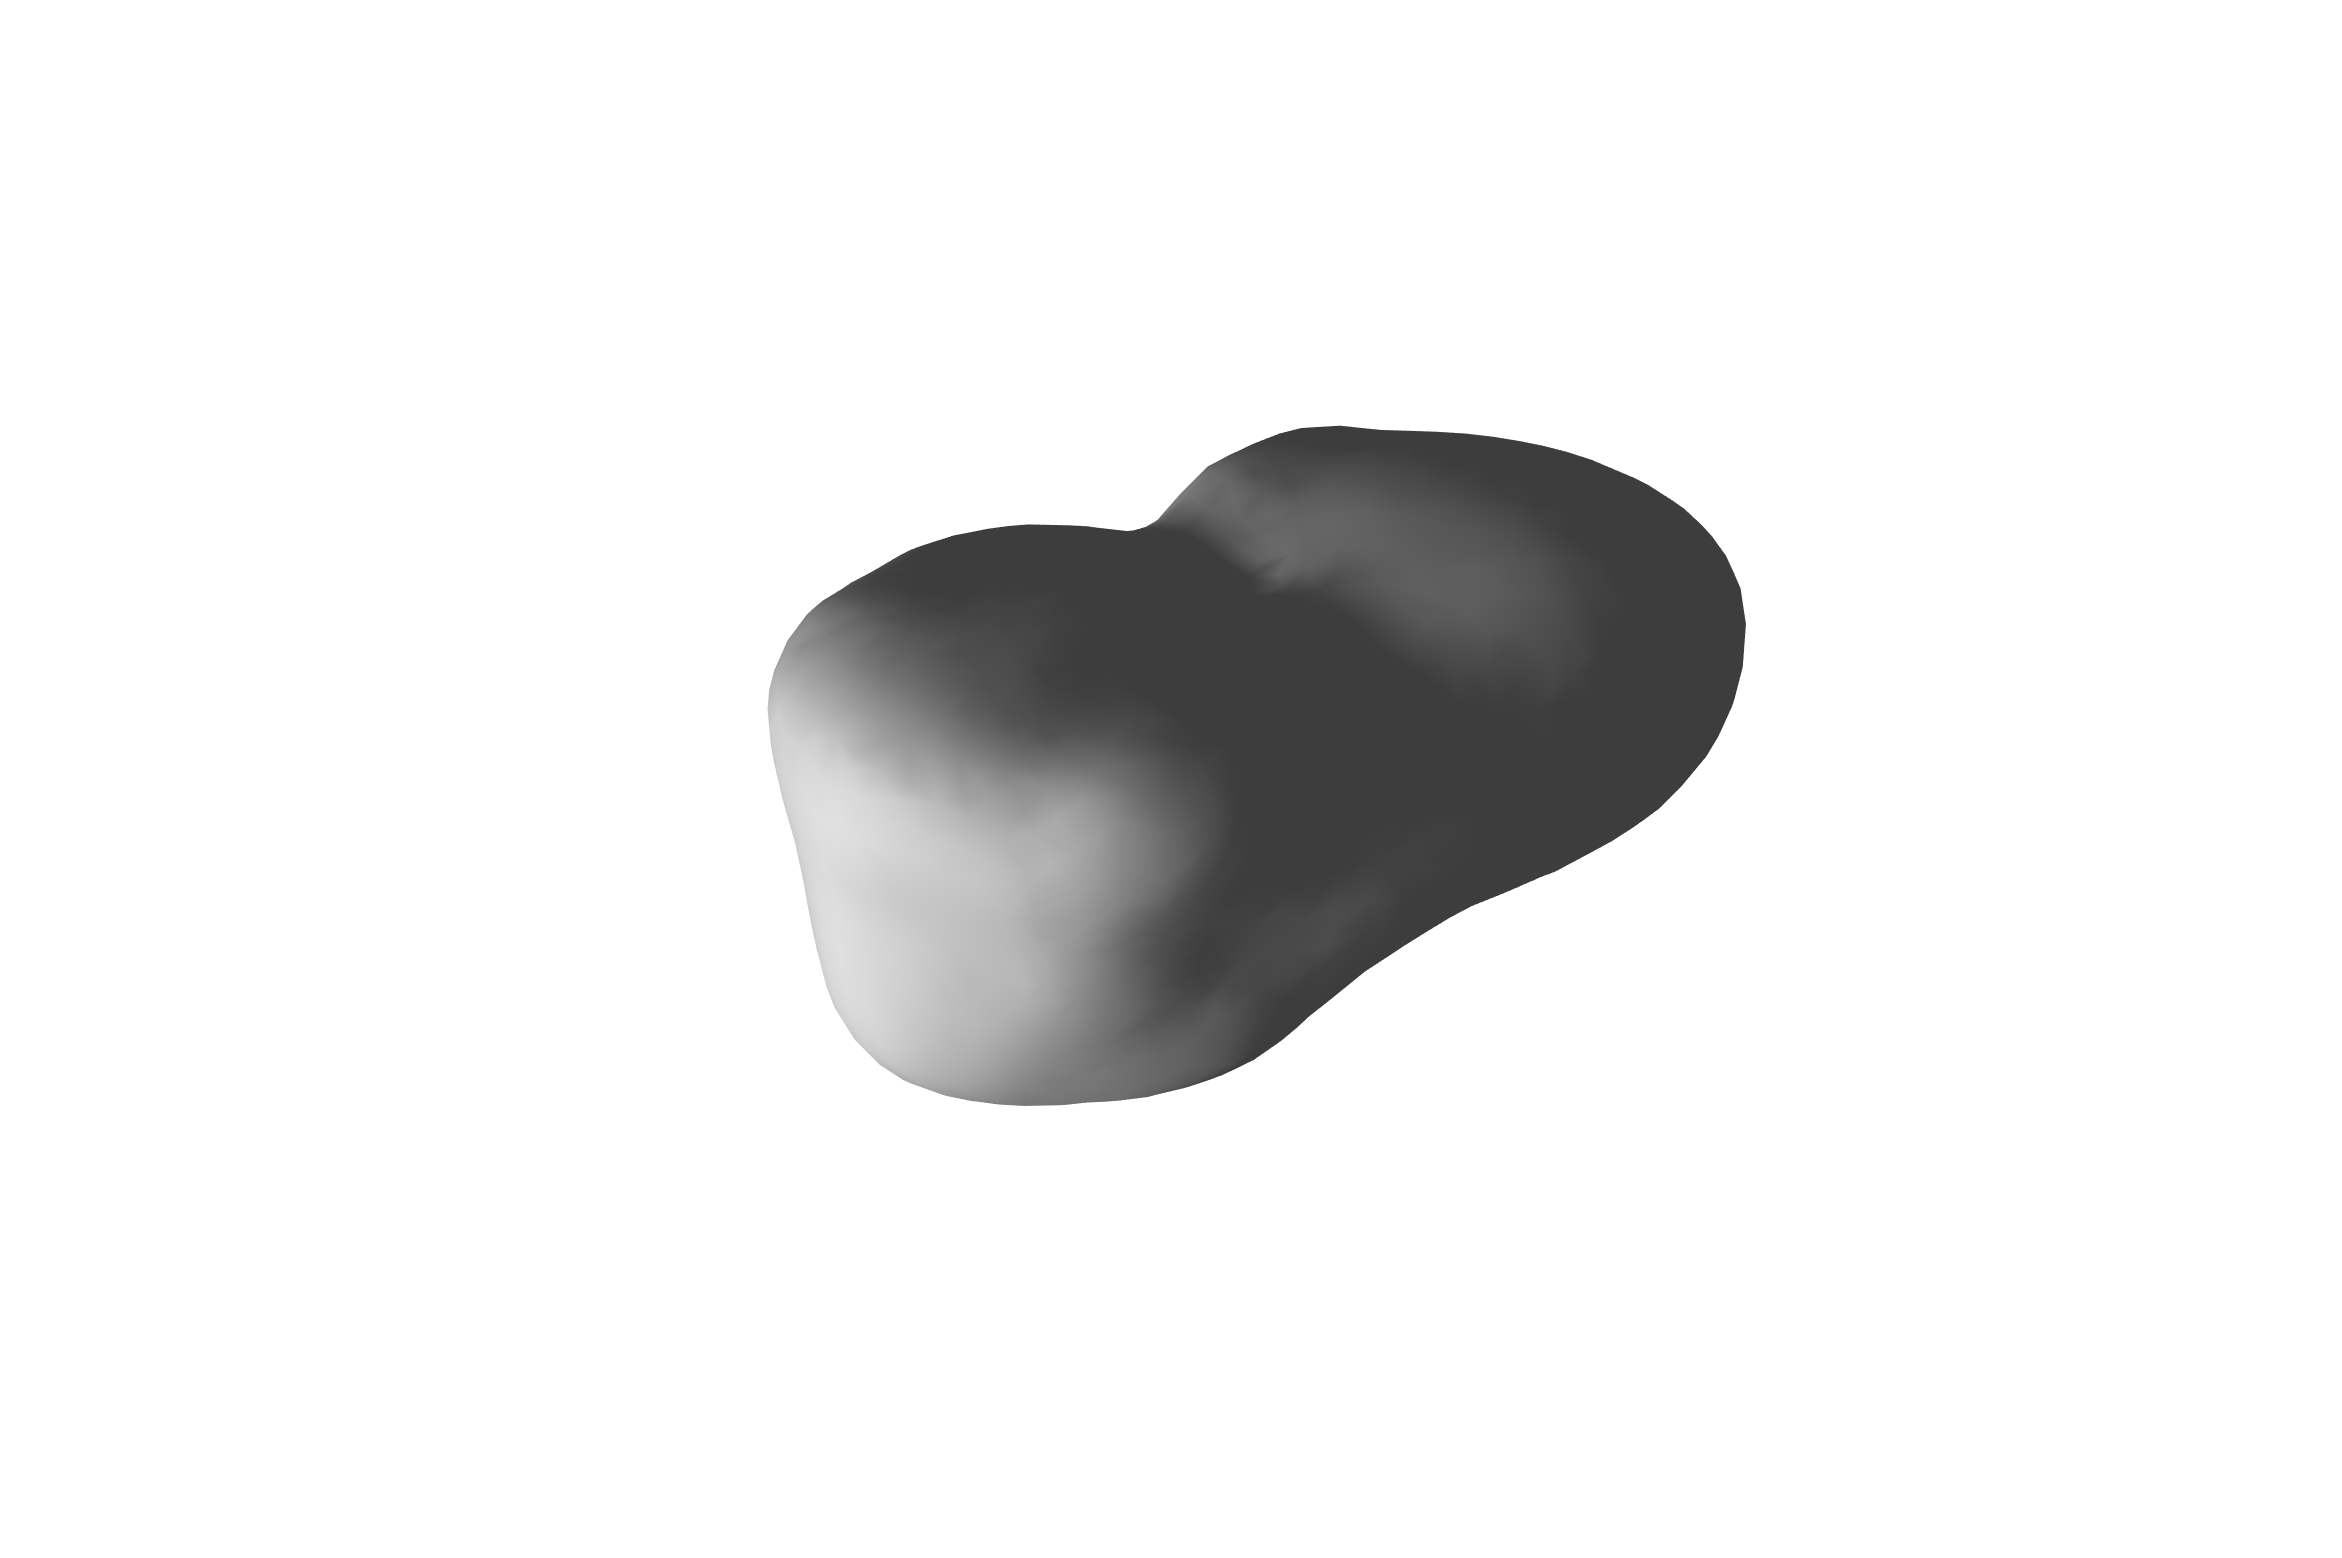
\includegraphics[trim={8cm 3cm 7cm 3cm},clip,width=0.5\columnwidth]{figures/castalia.pdf}
			\caption*{Asteroid 4769 Castalia}
		\end{figure}
	\end{minipage}%end of right half of block

\end{block} % end of structure block

\begin{block}{Simulation Results} % results block
    \begin{minipage}[t]{0.5\columnwidth}
    \begin{itemize}
        \item Transfer between two periodic orbits of 4769 Castalia
        \begin{itemize}
            \item Thruster represents a current electric propulsion \( \approx \SI{600}{\milli\newton}\)
            \item Combining multiple iterations of the \Emph{rechability} computation allows for general transfers
        \end{itemize}
        \item Combining four iterations of the reachability set
        \begin{itemize}
            \item Each iteration of the reachability set enlarges the achievable states
            \item We choose a direction on the reachability set which lies closest to the target
            \[
                d = \sqrt{k_x \parenth{x_f - x_t }^2 + k_z \parenth{z_f - z_t }^2 + k_{\dot{x}}\parenth{\dot{x}_f - \dot{x}_t }^2 + k_{\dot{z}}\parenth{\dot{z}_f - \dot{z}_t }^2}
            \]
            \item This iterative approach avoids the difficulty in choosing accurate initial guesses for optimization
        \end{itemize}
    \end{itemize}
    \end{minipage}~
    \begin{minipage}[t]{0.5\columnwidth}
    \begin{itemize}
        \item \Emph{Optimal Control} is used to calculate the reachability set
            \[
            J = -\frac{1}{2} \left( \vecbf{x}(t_f) - \vecbf{x}_{n}(t_f)\right)^T Q \left( \vecbf{x}(t_f) - \vecbf{x}_{n}(t_f)\right) 
            \]
        \item Maximize the distance on the section using the low thrust propulsion
        \item Thruster magnitude is limited by physical system
        \[
            c(\vecbf{u}) = \vecbf{u}^T \vecbf{u} - u_m^2 \leq 0 
        \]
        \item Terminal constraints ensure intersection with the section
    \end{itemize}
        \begin{align*}\label{eq:terminal_constraints}
            \begin{split}
                m_1 &= y = 0  \\
                m_2 &= \parenth{\sin \phi_{1_{d}}} \parenth{ x_1^2 + x_2^2 + x_3^2 + x_4^2} - x_1^2 = 0 \\
                m_3 &= \parenth{\sin \phi_{2_{d}}} \parenth{ x_2^2 + x_3^2 + x_4^2} - x_2^2 = 0\\
                m_4 &= \parenth{\sin \phi_{3_{d}}} \parenth{ 2 x_3^2 + 2 x_3 \sqrt{x_4^2 + 2 x_4^2}} - x_3 - \sqrt{x_4^2 + x_3^2} = 0 
            \end{split}
        \end{align*}
    \end{minipage}

\begin{figure}[htbp] 
    \centering 
    \begin{subfigure}[htbp]{0.5\textwidth} 
        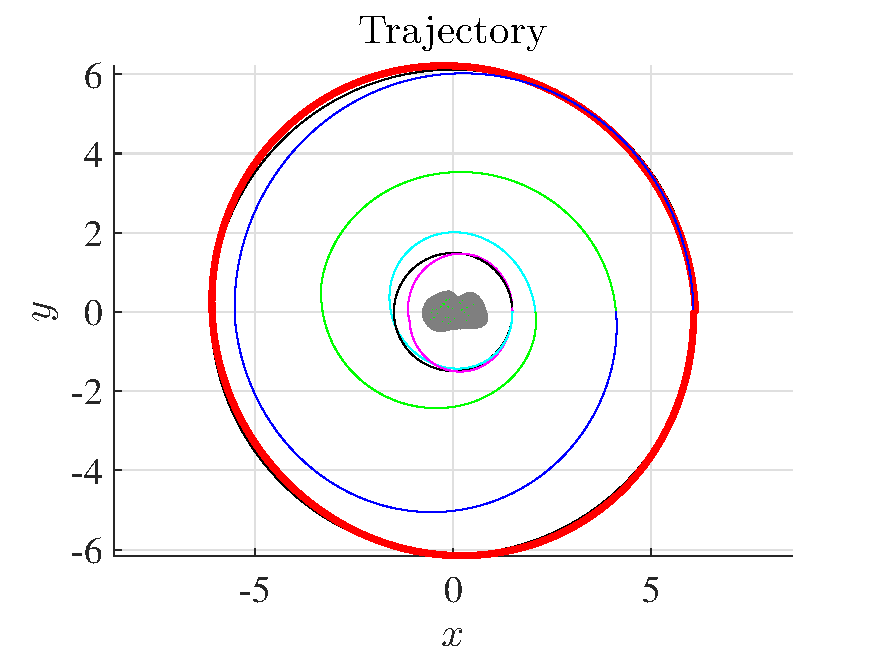
\includegraphics[width=\textwidth]{figures/trajectory.pdf} 
        \caption{Equatorial Transfer Trajectory}
    \end{subfigure}~ %add desired spacing between images, e. g. ~, \quad, \qquad, \hfill etc. %(or a blank line to force the subfigure onto a new line) 
    \begin{subfigure}[htbp]{0.5\textwidth} 
        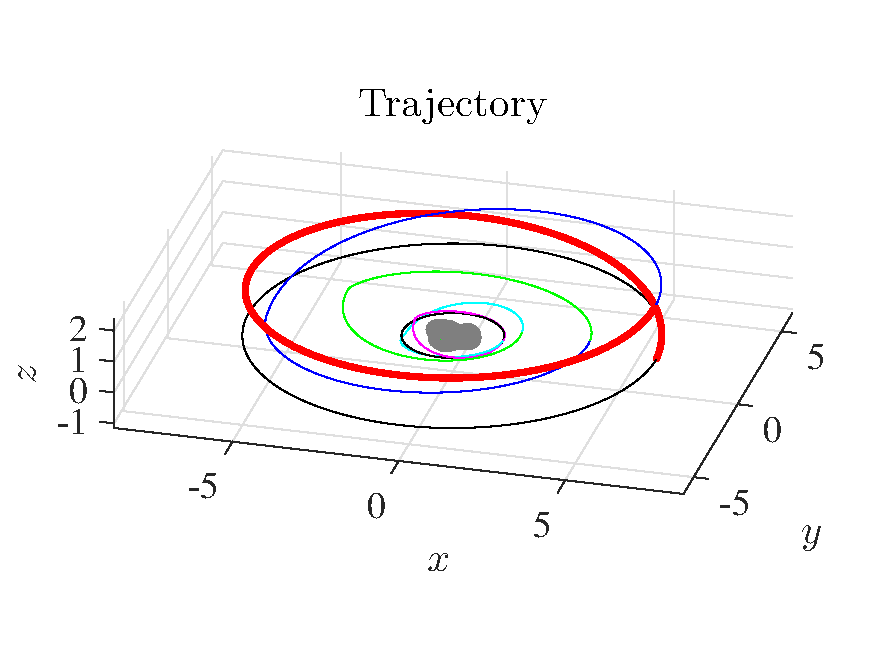
\includegraphics[width=\textwidth]{figures/trajectory_3d.pdf} 
        \caption*{3D Transfer Trajectory}
    \end{subfigure}
 
\end{figure}
    
\vspace{2cm}
\end{block} % end of results block

\end{column}


%-----------------------------------------------------------------------------------------
% THIRD (RIGHT) COLUMN
%---------------------------------------------------------------------------------------
\begin{column}{\onecolwidth} % third column start

\begin{block}{Reachability on the \Poincare section} % optimal control block

    \begin{figure}[htbp] 
        \centering 
            \begin{scaletikzpicturetowidth}{\columnwidth}
            \begin{tikzpicture}[tdplot_main_coords,
            poincare/.style={opacity=.2,very thick,fill=blue},
            orbit/.style={very thick,black},
            orbit hidden/.style={very thick,dashed},
            grid/.style={very thin,black},
            axis/.style={->,blue,thick},
            reachability/.style={thick,blue},scale=\tikzscale]

            % nodes for the poincare section
            \node[label=above:\(\Sigma\)] (upper_right) at (0,5,5) {};
            \node[] (upper_left) at (0,1,5) {};
            \node[] (lower_left) at (0,1,0) {};
            \node[] (lower_right) at (0,5,0) {};

            % draw poincare section
            \draw[poincare] (upper_right.center) -- (upper_left.center) -- (lower_left.center) -- (lower_right.center) -- (upper_right.center);

            % draw a periodic orbit
            \coordinate (center) at (0,0,2);
            \node[label=below:\(\vecbf{x}_n\)] (x0) at (0,3,2) {};
            % \node[label=below:\(\vecbf{x}_n\)] at (x0) {};
            \filldraw (x0) circle (3pt);

            % \tdplotdrawarc[orbit hidden]{(center)}{3}{90}{200}{}{};
            \tdplotdrawarc[orbit,<-]{(center)}{3}{-160}{90}{}{};

            % draw reachability set on the poincare section
            \coordinate (reach) at (0,4.5,2);
            \tdplotsetthetaplanecoords{90}

            \draw[tdplot_rotated_coords,grid] (x0) -- (reach);
            \draw[tdplot_rotated_coords,grid] (x0) -- ++(-45:1.5);

            \tdplotdrawarc[tdplot_rotated_coords,grid]{(x0)}{0.5}{-45}{90}{above}{\(\phi\)};

            % draw terminal state on reachability set
            \node[tdplot_rotated_coords,label=above:\(\vecbf{x}_f\)] (xf) at ($ (x0)+(-45:1.5) $) {};
            \filldraw (xf) circle (3pt);

            \node[tdplot_rotated_coords,label=below:\(J\)] at (xf) {};

            \tdplotdrawarc[tdplot_rotated_coords,reachability]{(x0)}{1.5}{0}{360}{}{};
            % place
            \end{tikzpicture}
            \end{scaletikzpicturetowidth}
            \caption*{Reachability set on a \Poincare section\label{fig:reachability_set}}
    \end{figure}


    \begin{itemize}
        \item \Emph{\Poincare} map is a useful tool in the analysis of dynamical systems
        \begin{itemize}
            \item Enables visualization of complicated systems - intrinsic structure becomes visible to the engineer
            \item Rather than considering the entire state (6D position and velocity) we simply investigate the intersections with a lower dimensional space
            \item This reduces the complexity of analyzing the dynamics and allows for visualization of highly complex dynamic interactions
        \end{itemize} 
        \item A periodic orbit on the \Poincare map is identified by fixed points \( \vecbf{x}_n\)
        \item Using the low-thrust propulsion system of the spacecraft we can enlarge the space that is achievable 
        \begin{itemize}
            \item \Emph{Reachability Set} - the set of states which are attainable subject to the constraints of the system
            \item The thruster of the spacecraft is used to design a transfer trajectory by repeatedly maximizing the reachability set
            \item Thruster allows us to depart from the fixed orbit and intersect at a new state \( \vecbf{x}_f\)
        \end{itemize}
        \item \Emph{Reachability Set} is computed on the \Poincare section and provides additional insight
        \begin{itemize}
            \item Spacecraft can only move to areas inside of the reachable set
        \end{itemize}
    \end{itemize}

\end{block} % end of optimal control block

\begin{block}{Conclusions} % conclusion
	\begin{itemize}
		\item Demonstrate a transfer around an asteroid using multiple \Emph{reachability sets}
        \begin{itemize}
            \item Each reachability set moves the spacecraft towards the target
        \end{itemize}
        \item Alleviates the need for selecting accurate initial guesses 
		\item Automatically gain insight into the feasible region of motion for the spacecraft
        \item Future work will extend this principle to landing trajectories on asteroids
        \begin{itemize}
            \item Irregular shape of asteroids requires innovative techniques for controlling both position and orientation
            \item Nonlinear control allows for the exploitation of the coupled dynamics
            \item Complex dynamics requires accurate integration schemes - \Emph{Variational Integrators}
        \end{itemize}
        \item Successful extension of previous work in the circular restricted three-body problem
	\end{itemize}
\end{block} % conclusion
\end{column}  % third column end

\end{columns} % end of all columns in poster
\end{frame} % end of enclosing frame
\end{document}